\section{Exploración Univariada}\label{univariada}




Teniendo en cuenta queel estudio se hizo para los 32 departamentos de Colombia

% Table created by stargazer v.5.2.2 by Marek Hlavac, Harvard University. E-mail: hlavac at fas.harvard.edu
% Date and time: vie., jun. 29, 2018 - 7:03:09 p.m.
\begin{table}[!htbp] \centering 
  \caption{Medidas estadísticas} 
  \label{stats} 
\begin{tabular}{@{\extracolsep{5pt}}lccccc} 
\\[-1.8ex]\hline 
\hline \\[-1.8ex] 
Statistic & \multicolumn{1}{c}{Mean} & \multicolumn{1}{c}{Median} & \multicolumn{1}{c}{St. Dev.} & \multicolumn{1}{c}{Min} & \multicolumn{1}{c}{Max} \\ 
\hline \\[-1.8ex] 
IDH & 0.802 & 0.804 & 0.042 & 0.691 & 0.879 \\ 
Poblacion.Cabecera & 1,196,730.000 & 717,197 & 1,982,287.000 & 13,090 & 10,070,801 \\ 
Poblacion.Resto & 360,590.300 & 268,111.5 & 331,887.600 & 21,926 & 1,428,858 \\ 
Poblacion.Total & 1,557,320.000 & 1,028,429 & 2,202,522.000 & 43,446 & 10,985,285 \\ 
\hline \\[-1.8ex] 
\end{tabular} 
\end{table} \centering




\begin{figure}[h]
\centering
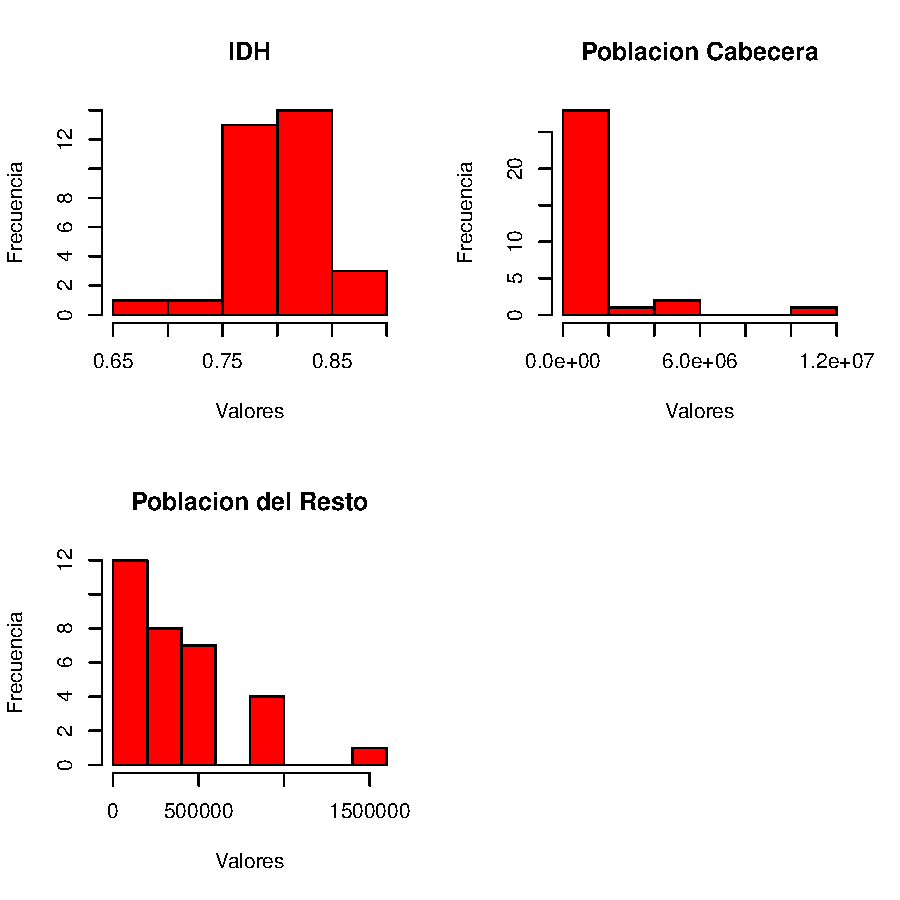
\includegraphics{univariada-hist}
\caption{Distribuci?n de Indicadores}
\label{hist}
\end{figure}

Si quieren normalizar dado el sesgo de las poblaciones, se tranforma con logaritmo en case 10 y quedaria asi:

\begin{figure}[h]
\centering
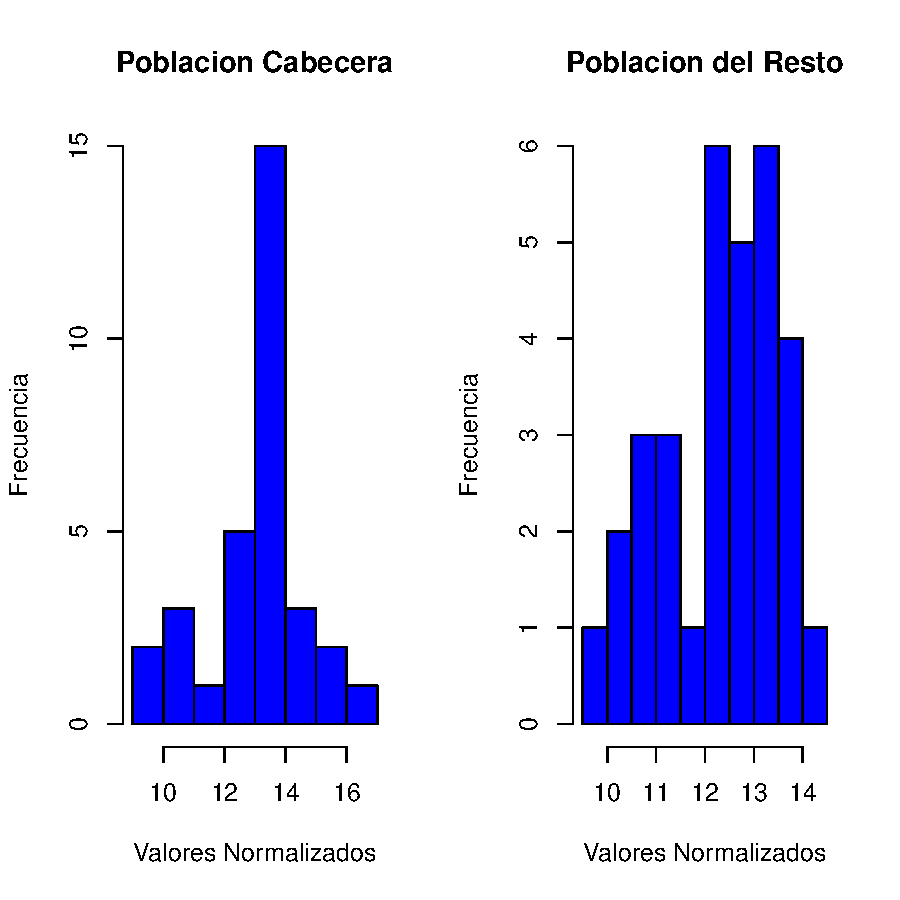
\includegraphics{univariada-hist1}
\caption{Distribuci?n de Indicadores de Poblaciones Normalizado}
\label{hist1}
\end{figure}

\endinput
